% ************ Chapter 4 ************
%\renewcommand{\chaptername}{Chapter}

\chapter{Desenho}
\label{cap:4}
\emph{Este capítulo incide na apresentação da forma como a framework Solid está até ao momento estruturada e como será estruturada a nova arquitetura proposta.}

\section{Arquitetura Actual}

O Solid é um projeto open-source, desenvolvido principalmente por uma comunidade criada e ativamente impulsionada por Tim Berners-Lee. Esta comunidade dedica os seus esforços principalmente no desenvolvimento do POD como um todo, bem como documentação e ferramentas que permitem uma mais fácil integração da solução de novas aplicações. Desta forma,a arquitetura actual prende-se a uma estrutura monólito, na qual existe apenas um processo responsável por arrancar todo o servidor POD.

\section{Arquitetura Proposta}
A arquitetura atual centraliza muitas camadas importantes no mesmo processo, afetando assim a escalabilidade, e pode consequentemente condenar o sucesso desta framework (c.f seccção 2.1.1).

Existe, desta forma, espaço para evoluir para uma arquitetura orientada a micro-serviços, potencialmente assente na divisão por capacidades de negócio, resumindo-se estas às seguintes:
\begin{itemize}
    \item  Autenticar utilizadores - Esta autenticação consiste sobretudo em garantir que a autenticidade do utilizador e conferir acesso da aplicação cliente ao seu WebID;
    \item Autorizar acesso de utilizador a determinado recurso - Deve ser possível consultar, alterar e criar novas regras de acesso a recursos num qualquer POD existente;
    \item Aceder e efetuar operações sobre recursos - O utilizador deve conseguir (se autenticado e autorizado) efectuar operações sobre recursos.
\end{itemize}

Desta forma, a arquitetura proposta terá em consideração a separação da plataforma atual em 3 componentes:
\begin{description}
    \item ID -  Será a camada responsável pela autenticação do utilizador, esta autenticação.
    \item ACL - Camada responsável pela autorização.
    \item LDP - Camadas responsável pelo acesso a recursos.
\end{description}


Tendo por base as camadas apresentadas, seguem-se duas arquiteturas (\ref{subsection:arquitetura_1} - Arquitetura baseada em pedidos HTTP e \ref{subsection:arquitetura_2} - Arquitetura baseada em pedidos HTTP e eventos) com potencial para migração da plataform Solid para micro-serviços.

\subsection{Arquitetura baseada em pedidos HTTP} \label{subsection:arquitetura_1}

Esta arquitetura introduz o conceito de API Gateway como o ponto de entrada para todos o micro-serviços. Este padrão (c.f em \ref{api_gateway} permite, desta forma, encapsular os diferentes serviços em pedidos \emph{HTTP}, que reencaminham o pedido para o serviço mais indicado. Esta abstração oferece vantagens como:

\begin{itemize}
    \item Escalabilidade - No futuro, a separação dos serviços existentes ou a criação de novos, não adicionará complexidade para além da de alterar as regras de encaminhamento na API Gateway. Esta camada, Podendo inclusive ser utilizada para migrações controladas de tráfego entre serviços legados e novos.
    
    \item Segurança - A camada da API Gateway deverá centralizar responsabilidades como \emph{throttling} e inibição de tráfego com base em características do pedido (por exemplo IP de origem). O componente ID, não deverá estar "escondido" atrás da API Gateway, porque se trata de uma camada que deverá estar visível para o cliente, devendo esta ser utilizada para obter posteriormente acesso às funcionalidades expostas através da API Gateway.
\end{itemize}

\subsubsection{Diagrama de componentes}
\begin{figure}[h]
    \begin{center}
    % Requires \usepackage{graphicx}
    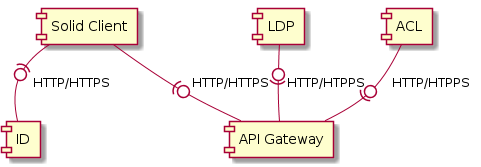
\includegraphics[width=1 \textwidth]{figures/component_diagram_2.png}
    \caption{Diagrama de Componentes Arquitetura 1}
    \end{center}
\end{figure}
\pagebreak

\subsection{Arquitetura baseada em pedidos HTTP e eventos} \label{subsection:arquitetura_2}

Esta arquitetura mantêm o conceito de API Gateway, mas introduz a adoção de mecanismos de troca de mensagens assíncrona (c.f. em \ref{troca_mensagens_assincrona}) como possível forma de actualização assíncrona das permissões de acesso a recursos no LDP.

Na prática o que isto permite é que a leitura das permissões seja independente da escrita das mesmas. E, desta forma, aplica-se o padrão CQRS (Command Query Responsability Segregation) (c.f secção \ref{cqrs}, contribuindo para um menor acoplamento entre o LDP e o ACL. Este conceito introduz indiretamente um outro: \emph{Eventual Consistency}, este por sua vez consiste na assunção de que alterações a um determinado modelo eventualmente induzirão num estado consistente no sistema como um todo. De acordo com o teorema de CAP (c.f secção \ref{_theorem}), consistência é o parâmetro que devemos abdicar para conseguirmos escalabilidade e tolerância a falhas.

A utilização da arquitetura permite também a adoção do padrão \emph{Event Sourcing} (c.f. secção \ref{event_sourcing}, este consiste na persistência dos eventos de alteração de estado e permite que o estado do sistema seja obtido a qualquer momento pela "soma" das alterações de estado a que o mesmo foi sujeito.

\begin{figure}[H]
    \begin{center}
    % Requires \usepackage{graphicx}
    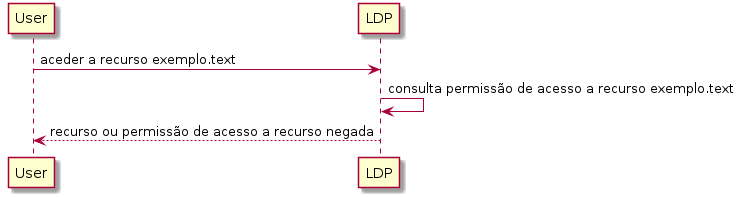
\includegraphics[width=1 \textwidth]{figures/arquitetura_2_access_resource}
    \caption{Diagrama de Sequência arquitetura baseada em pedidos HTTP e eventos - alterar permissão a recurso}
    \end{center}
\end{figure}

\begin{figure}[H]
    \begin{center}
    % Requires \usepackage{graphicx}
    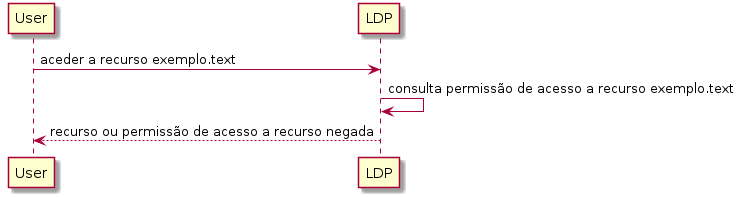
\includegraphics[width=1 \textwidth]{figures/arquitetura_2_access_resource}
    \caption{Diagrama de Sequência arquitetura baseada em pedidos HTTP e eventos - aceder recurso}
    \end{center}
\end{figure}


\subsubsection{Diagrama de componentes}
\begin{figure}[H]
    \begin{center}
    % Requires \usepackage{graphicx}
    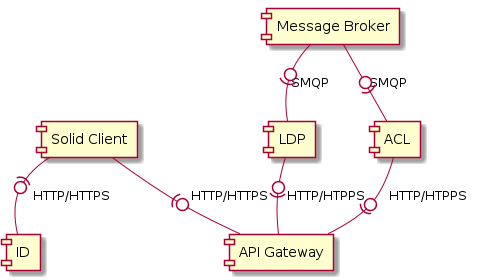
\includegraphics[width=1 \textwidth]{figures/component_diagram.png}
    \caption{Diagrama de Componentes arquitetura baseada em pedidos HTTP e eventos}
    \end{center}
\end{figure}

\subsection{Análise comparativa}
Ambas as arquiteturas apresentadas compreendem uma migração para micro-serviços, sustentada numa separação em serviços baseada em capacidades de negócio.

A grande diferença entre as duas é a introdução da componente Message Broker na arquitetura baseada em pedidos HTTP e eventos, este factor adiciona complexidade, mas por outro lado, garante um maior desacoplamento entre a componente LDP e a componente ACL e garante também uma diminuição da latência na obtenção de um recurso. O ponto negativo desta abordagem é a complexidade que adiciona ao desenvolvimento e ao processo de deploy de um POD como um todo, na medida em que a sua infraestrutura será mais robusta e complexa também.







